
%% overclocking_tcad.tex
%% by Kan Shi


%\usepackage{times,epsfig,amsfonts,bm}
%\usepackage{pdflscape}
%\usepackage{afterpage}
%\usepackage{algorithm}
%\usepackage{algorithmic}
%\usepackage{fmtcount,threeparttable, setspace, nicefrac}
%\usepackage[dvips]{color}
%\usepackage{amsthm}

\documentclass[journal]{IEEEtran}
\usepackage{cite}

\ifCLASSINFOpdf
  \usepackage[pdftex]{graphicx}
  % declare the path(s) where your graphic files are
  % \graphicspath{{../pdf/}{../jpeg/}}
  % and their extensions so you won't have to specify these with
  % every instance of \includegraphics
  % \DeclareGraphicsExtensions{.pdf,.jpeg,.png}
\else
  % or other class option (dvipsone, dvipdf, if not using dvips). graphicx
  % will default to the driver specified in the system graphics.cfg if no
  % driver is specified.
  \usepackage[dvips]{graphicx}
  % declare the path(s) where your graphic files are
  \graphicspath{{../Figures/}}
  % and their extensions so you won't have to specify these with
  % every instance of \includegraphics
  \DeclareGraphicsExtensions{.eps}
\fi
\usepackage{epstopdf}


\usepackage{multirow}
\usepackage{amssymb}
\usepackage[cmex10]{amsmath}
%\usepackage{algorithmic}
%\usepackage{array}
\usepackage[tight,footnotesize]{subfigure}
\usepackage{stfloats}



\begin{document}

\title{Title}

\author{Kan~Shi,
        David~Boland,~\IEEEmembership{Member,~IEEE,}
        and~George~A.~Constantinides,~\IEEEmembership{Senior~Member,~IEEE}% <-this % stops a space
	\thanks{K. Shi, D. Boland and G. A. Constantinides are with the Department of Electrical and Electronic Engineering, Imperial College London, London, SW7 2BT, U.K. (email: \{k.shi11, david.boland03, g.constantinides\}@imperial.ac.uk)}%
	%\thanks{M. Shell is with the Department of Electrical and Computer Engineering, Georgia Institute of Technology, Atlanta,GA, 30332 USA e-mail: (see http://www.michaelshell.org/contact.html).}% <-this % stops a space
%\thanks{J. Doe and J. Doe are with Anonymous University.}% <-this % stops a space
\thanks{Manuscript received April 19, 2005; revised December 27, 2012.}}

% note the % following the last \IEEEmembership and also \thanks -
% these prevent an unwanted space from occurring between the last author name
% and the end of the author line. i.e., if you had this:
%
% \author{....lastname \thanks{...} \thanks{...} }
%                     ^------------^------------^----Do not want these spaces!
%
% a space would be appended to the last name and could cause every name on that
% line to be shifted left slightly. This is one of those "LaTeX things". For
% instance, "\textbf{A} \textbf{B}" will typeset as "A B" not "AB". To get
% "AB" then you have to do: "\textbf{A}\textbf{B}"
% \thanks is no different in this regard, so shield the last } of each \thanks
% that ends a line with a % and do not let a space in before the next \thanks.
% Spaces after \IEEEmembership other than the last one are OK (and needed) as
% you are supposed to have spaces between the names. For what it is worth,
% this is a minor point as most people would not even notice if the said evil
% space somehow managed to creep in.



% The paper headers
\markboth{Journal of \LaTeX\ Class Files,~Vol.~11, No.~4, December~2012}%
{Shell \MakeLowercase{\textit{et al.}}: Bare Demo of IEEEtran.cls for Journals}

\maketitle

% As a general rule, do not put math, special symbols or citations
% in the abstract or keywords.
\begin{abstract}
The abstract.
\end{abstract}

\begin{IEEEkeywords}

\end{IEEEkeywords}


% For peer review papers, you can put extra information on the cover
% page as needed:
% \ifCLASSOPTIONpeerreview
% \begin{center} \bfseries EDICS Category: 3-BBND \end{center}
% \fi
%
% For peerreview papers, this IEEEtran command inserts a page break and
% creates the second title. It will be ignored for other modes.
\IEEEpeerreviewmaketitle



\section{Introduction}
% The very first letter is a 2 line initial drop letter followed
% by the rest of the first word in caps.
%
% form to use if the first word consists of a single letter:
% \IEEEPARstart{A}{demo} file is ....
%
% form to use if you need the single drop letter followed by
% normal text (unknown if ever used by IEEE):
% \IEEEPARstart{A}{}demo file is ....
%
% Some journals put the first two words in caps:
% \IEEEPARstart{T}{his demo} file is ....
%
% Here we have the typical use of a "T" for an initial drop letter
% and "HIS" in caps to complete the first word.
\IEEEPARstart{T}{his} demo file is intended to serve as a ``starter file''
for IEEE journal papers produced under \LaTeX\ using
IEEEtran.cls version 1.8 and later.
% You must have at least 2 lines in the paragraph with the drop letter
% (should never be an issue)
I wish you the best of success.

\hfill mds

\hfill December 27, 2012

\subsection{Subsection Heading Here}
Subsection text here.


\subsubsection{Subsubsection Heading Here}
Subsubsection text here.
\section{Ripple Carry Adder}\label{section_RCA}
\subsection{Adder Structures in FPGAs}
%something about fast carry logic in FPGA and pictures
Adders serve as a key building block for arithmetic operations. Generally speaking, the ripple carry adder (RCA) is the most straightforward and widely used adder structure. As such, the philosophy of our approach is first exemplified with the analysis of a RCA. We later describe how this methodology can be extended to other arithmetic operators in Section~\ref{section_CCM} by discussing  the CCM that is commonly used in DSP applications and numerical algorithms.

Typically the maximum frequency of a RCA is determined by the longest carry propagation. Consequently, modern FPGAs offer built-in architectures for very fast ripple carry addition. For instance, the Altera Cyclone series uses fast tables~\cite{AlteraCyclone} while the Xilinx Virtex series employs dedicated multiplexers and encoders for the fast carry logic~\cite{Virtex6}. Figure~\ref{FPGA adder} illustrates the structure of an $n$-bit RCA, which is composed of $n$ serial-connected full adders (FAs) and utilizes the internal fast carry logic of the Virtex-6 FPGA.

While the fast carry logic reduces the time of each individual carry-propagation delay, the overall delay of carry-propagation will eventually overwhelm the delay of sum generation of each LUT with increasing operand word-lengths. For our initial analysis, we assume that the carry propagation delay of each FA is a constant value $\mu$, which is a combination of logic delay and routing delay, and hence the critical path delay of the RCA is $\mu_{RCA}=n\mu$, as shown in~Figure~\ref{FPGA adder}. For an $n$-bit RCA, it follows that if the sampling period $T_S$ is greater than $\mu_{RCA}$, correct results will be sampled. If, however, $T_S<\mu_{RCA}$, intermediate results will be sampled, potentially generating errors.
%
\begin{figure}[t]
  \centering
  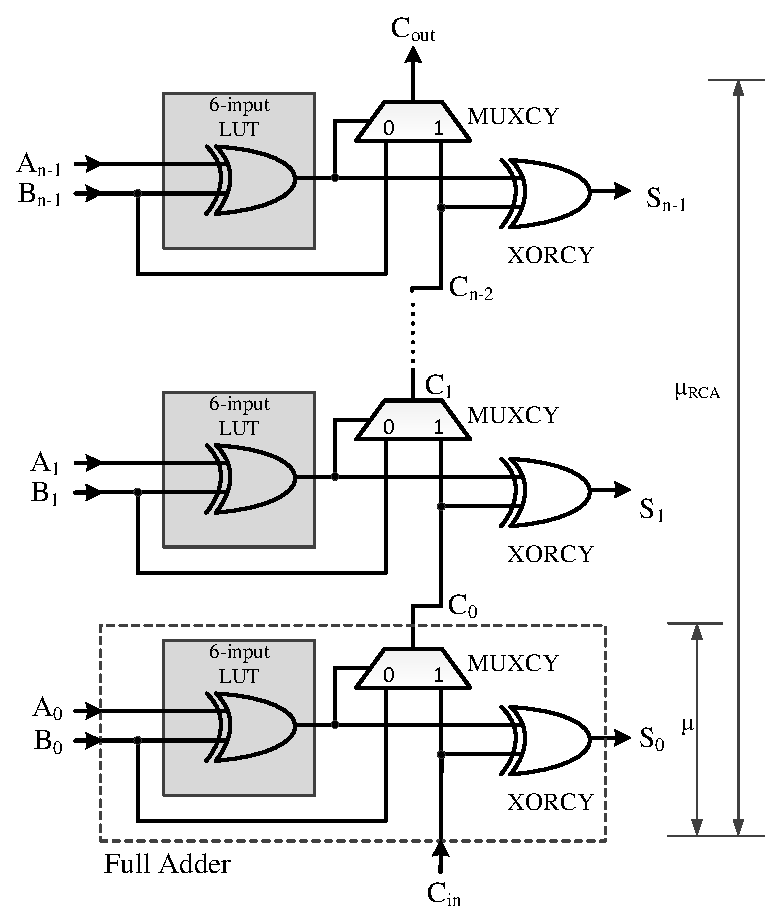
\includegraphics[width=3in]{./Figures/FastCarryLogic3.eps}
%  \vspace{-2ex}
  \caption{An $n$-bit ripple carry adder in Virtex-6 FPGA.}
  \label{FPGA adder}
  %\vspace{-3.5ex}
\end{figure}

In the following sections, we consider two methods that would allow the circuit to run at a frequency higher than $1/{T_S}$. The first is a traditional circuit design approach where operations occur without timing violations. To this end, the operand word-length is truncated in order to meet the timing requirement. This process results in truncation or roundoff error. In our proposed new scenario, circuits are implemented with greater word-length, but are clocked beyond the safe region so that timing violations sometimes occur. This process generates ``overclocking error''.

 %We note that it may be possible to operate at a higher clock frequency than $1/T_{S}$ by using alternative adder structures, such as carry-select adder and carry lookahead adder. However, the effectiveness of these techniques is limited in FPGAs due to the build-in structures for the acceleration of carry propagation. In addition, such techniques will require substantial extra silicon area.

\subsection{Probabilistic Model of Truncation Error}
For ease of discussion, we assume that the input to our circuit is a fixed point number scaled to lie in the range $[-1,1)$. For our initial analysis, we assume every bit of each input is uniformly and independently generated. However, this assumption will be relaxed in Section~\ref{Section_Experiments} where the predictions are verified using real image data. The errors at the output are evaluated in terms of the absolute value and the probability of their occurring. These two metrics are combined as the error expectation.

If the input signal of a circuit is $k$ bits, truncation error occurs when the input signal is truncated from $k$ bits to $n$ bits. Under this premise, the mean value of the truncated bits at signal input ($E_{Tin}$) is given by (\ref{ET at single input}).
%
%\vspace{-1ex}
\begin{eqnarray}\label{ET at single input}
%\small
%\footnotesize
%\scriptsize
  E_{Tin}=\frac{1}{2}\sum_{i=n+1}^{k}2^{-i}=2^{-n-1}-2^{-k-1}
%  \vspace{-1ex}
\end{eqnarray}
%\normalsize

Since we assume there are two mutually independent inputs to the RCA, the overall expectation of truncation error for the RCA is given by (\ref{TruncationError}).
%
%\vspace{-1ex}
\begin{eqnarray}\label{TruncationError}
%\small
%\footnotesize
  E_T=\left\{
    \begin{matrix}
        2^{-n}-2^{-k}, & \textrm{if $n<k$}\\
        0, & \textrm{otherwise}
    \end{matrix}
  \right.
\end{eqnarray}
%\normalsize

\subsection{Probabilistic Model of Overclocking Error}
\subsubsection{Generation of Overclocking Error}\label{subsub:Generation of Overclocking Error}
For a given $T_S$, the maximum length of error-free carry propagation is described by~(\ref{Max.length of carry chain}), where $f_S$ denotes the sampling frequency.
%
%\vspace{-1ex}
\begin{eqnarray}\label{Max.length of carry chain}
%\small
%\footnotesize
%\scriptsize
    b:=\left\lceil \frac{T_S}{\mu} \right\rceil=\left\lceil \frac{1}{\mu\cdot f_S}\right\rceil
\end{eqnarray}
%\normalsize

However, since the length of an actual carry chain during execution is dependent upon input patterns, in general, the worst case may occur rarely. To determine when this timing constraint is not met and the size of the error in this case, we expand standard results~\cite{DigitalICDesign} to the following statements, which examine carry generation, propagation and annihilation, as well as the corresponding summation results of a single bit $i$, according to the relationship between its input patterns $A_i$ and $B_i$:
%
 \begin{itemize}
   \item If $\!A_i\!=\!B_i\!=1$, a new carry chain is generated at bit $i$, and $S_i\!=\!C_{i-1}$;
   \item If $A_i\neq B_i$, the carry propagates for this carry chain at bit $i$, and $S_i\!=\!0$;
   \item If $\!A_i\!=\!B_i$, the current carry chain annihilates at bit $i$, and $S_i\!\!=\!\!1$.
 \end{itemize}

\subsubsection{Absolute Value of Overclocking Error}
For an $n$-bit RCA, let $C_{tm}$ denote the carry chain generated at bit $S_t$ with the length of $m$ bits. For a certain $f_S$, the maximum length of error-free carry propagation, $b$, is determined through (\ref{Max.length of carry chain}). The presence of overclocking error requires $m>b$. Since the length of carry chain cannot be greater than $n$, parameters $t$ and $m$ are bounded by (\ref{t_RCA}) and (\ref{m_RCA}):
%
%\vspace{-1ex}
\begin{align}
%\small
%\footnotesize
%\scriptsize
  \label{t_RCA}  0&\leq t \leq n-b\\
    b&<m\leq n+1-t      \label{m_RCA}
%    \vspace{-1ex}
\end{align}
%\normalsize

For $C_{tm}$, correct results will be generated from bit $S_t$ to bit $S_{t+b-1}$. Hence the absolute value of error seen at the output, normalized to the MSB ($2^n$), is given by (\ref{Output Error}), where $\hat{S_i}$ and $S_i$ denote the actual and error-free output of bit $i$ respectively.
%
%\vspace{-1ex}
\begin{eqnarray}\label{Output Error}
%\small
%\footnotesize
    e_{tm}=\frac{\left|\sum_{i=t+b}^{n}(S_i-\hat{S_i})\cdot 2^i\right|}{2^n}
%    \vspace{-1ex}
\end{eqnarray}
%\normalsize

$S_i$ and $\hat{S_i}$ can be determined using the equations from the previous statements in Section~\ref{subsub:Generation of Overclocking Error}. In the error-free case, the carry will propagate from bit $S_t$ to bit $S_{t+m-1}$, and we will obtain $S_{t+b}=S_{t+b+1}=\cdots=S_{t+m-2}=0$ for carry propagation, and $S_{t+m-1}=1$ for carry annihilation. However, when a timing violation occurs, the carry will not propagate through all these bits. Substituting these values into (\ref{Output Error}) yields (\ref{etm}). Interestingly, the value of overclocking error has no dependence on the length of carry chain $m$.
%
%Instead, $\hat{S}_{t+b}=\hat{S}_{t+b+1}=\cdots=\hat{S}_{t+m-2}=1$ and $\hat{S}_{t+m-1}=0$. It is worth noting that these expressions are obtained based on the assumption that all the internal bits are initialized to zero.
%
\begin{eqnarray}\label{etm}
%\small
%\footnotesize
  e_{tm}=\frac{\left|2^{t+m-1}-2^{t+m-2}-\dots-2^{t+b}\right|}{2^n}=2^{t+b-n}
\end{eqnarray}
%\normalsize

\subsubsection{Probability of Overclocking Error}
The carry chain $C_{tm}$ occurs when there is a carry generated at bit $t$, a carry annihilated at bit $t+m-1$ and the carry propagates in between. Consequently, its probability $P_{tm}$ is given by (\ref{Ptm_RCA}).
%
%\vspace{-1ex}
\begin{eqnarray}\label{Ptm_RCA}
%\small
%\footnotesize
  P_{tm}=P_{(A_t=B_t=1)}P_{(A_{t+m-1}=B_{t+m-1})}\cdot \prod_{i=t+1}^{t+m-2}P_{(A_i\neq B_i)}
%  \vspace{-1ex}
\end{eqnarray}
%\normalsize
Under the assumption that $A$ and $B$ are mutually independent and uniformly distributed, we have $P_{(A_i=B_i=1)}=1/4$, $P_{(A_i\neq B_i)}=1/2$ and $P_{(A_i=B_i)}=1/2$, so $P_{tm}$ can be obtained by~(\ref{Ptm2}). Note that~(\ref{Ptm2}) takes into account the carry annihilation always occurs when $t+m-1=n$.
%\vspace{-1ex}
%
\begin{eqnarray}\label{Ptm2}
%\small
%\footnotesize
    P_{tm}=\left\{\begin{array}{ll}
      (1/2)^{m+1} & \textrm{if $t+m-1<n$}\\
      (1/2)^{m} & \textrm{if $t+m-1=n$}
    \end{array} \right.
%    \vspace{-1ex}
\end{eqnarray}
%\normalsize

\subsubsection{Expectation of Overclocking Error}
Expectation of overclocking error can be expressed by (\ref{Eo_exp}).
%
%\vspace{-1ex}
\begin{eqnarray}\label{Eo_exp}
%\small
%\footnotesize
%\scriptsize
    %E_O=\sum_{t=0}^{n-b}\sum_{m=b+1}^{n-t+1}P_{tm}\cdot e_{tm}
    E_O=\sum_{t}\sum_{m}P_{tm}\cdot e_{tm}
%    \vspace{-1ex}
\end{eqnarray}
%\normalsize
%
Using $P_{tm}$ and $e_{tm}$ from (\ref{etm}) and (\ref{Ptm2}) respectively, $E_O$ can be obtained by (\ref{Eo}).
%\vspace{-1ex}
\begin{eqnarray}\label{Eo}
%\small
%\footnotesize
      E_O=\left\{
        \begin{matrix}
            2^{-b}-2^{-n-1}, & \textrm{if $b\leq n$}\\
            0, & \textrm{otherwise}
        \end{matrix}
      \right.
%      \vspace{-1ex}
\end{eqnarray}
%\normalsize

\subsection{Comparison between Two Scenarios}
In the traditional scenario, the word-length of RCA must be truncated, using $n=b-1$ bits, in order to meet a given $f_S$. The error expectation is then given by (\ref{Eo_trad_RCA}).
%
\begin{eqnarray}\label{Eo_trad_RCA}
%\small
%\vspace{-1ex}
%\footnotesize
%\scriptsize
  E_{trad}=2^{-b+1}-2^{-k}
  \vspace{-1ex}
\end{eqnarray}
%\normalsize
Overclocking errors are allowed to happen in the second scenario, therefore the word-length of RCA is set to be equal to the input word-length, that is, $n=k$. Hence we obtain (\ref{Eo_new_RCA}) according to (\ref{Eo}).
%
\begin{eqnarray}\label{Eo_new_RCA}
%\vspace{-1ex}
%\small
%\footnotesize
%\scriptsize
  E_{new}=2^{-b}-2^{-k-1}
%  \vspace{-1ex}
\end{eqnarray}
%\normalsize

%
Comparing (\ref{Eo_new_RCA}) and (\ref{Eo_trad_RCA}), we have (\ref{Comparison RCA}). This equation indicates that by allowing timing violations, the overall error expectation of RCA outputs drops by a factor of 2 in comparison to traditional scenario. This provides the first hint that our approach is useful in practice.
%
\begin{eqnarray}\label{Comparison RCA}
%\vspace{-1ex}
%\small
%\footnotesize
%\scriptsize
  \frac{E_{new}}{E_{trad}}=\frac{2^{-b}-2^{-k-1}}{2^{-b+1}-2^{-k}}=\frac{1}{2}
\end{eqnarray}

\section{Constant Coefficient Multiplier}\label{section_CCM}

As another key primitive of arithmetic operations, CCM can be implemented using RCA and shifters. For example, operation $B=9A$ is equivalent to $B=A+8A=A+(A<<3)$, which can be built using one RCA and one shifter. We first focus on a single RCA and single shifter structure. We describe how more complex structures consisting of multiple RCAs and multiple shifters can be built in accordance with this baseline structure in Section~\ref{CCM_Multi}.

In this CCM structure, let the two inputs of the RCA be denoted by $A_S$ and $A_O$ respectively, which are both two's complement numbers. $A_S$ denotes the ``shifted signal", with zeros padded after LSB, while $A_O$ denotes the ``original signal" with MSB sign extension. For an $n$-bit input signal, it should be noted that an $n$-bit RCA is sufficient for this operation, because no carry will be generated or propagated when adding with zeros, as shown in Figure~\ref{CCM_fig}.
\begin{figure}[htbp]
  \centering
%  \vspace{-2ex}
  %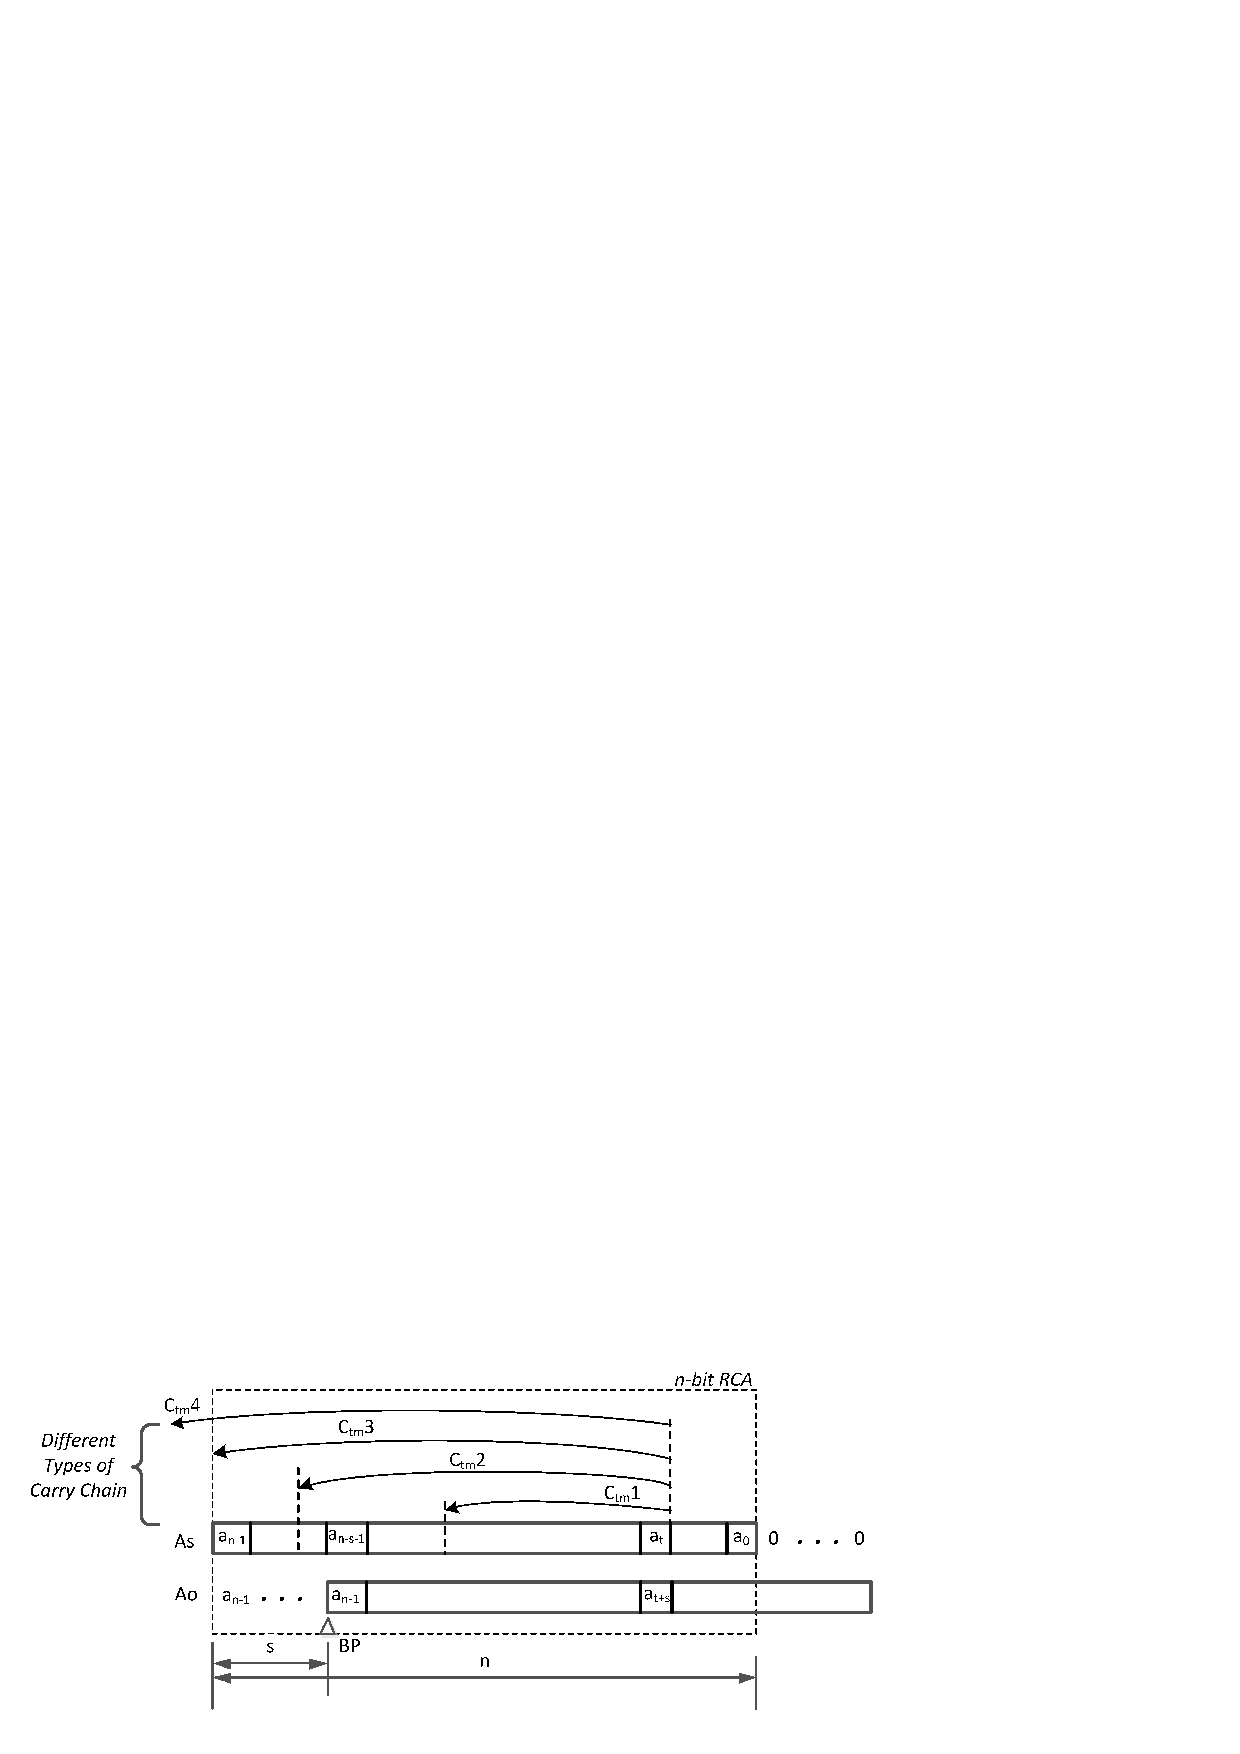
\includegraphics[width=3.5in]{./Figures/CCM_DataFlow3.pdf}
  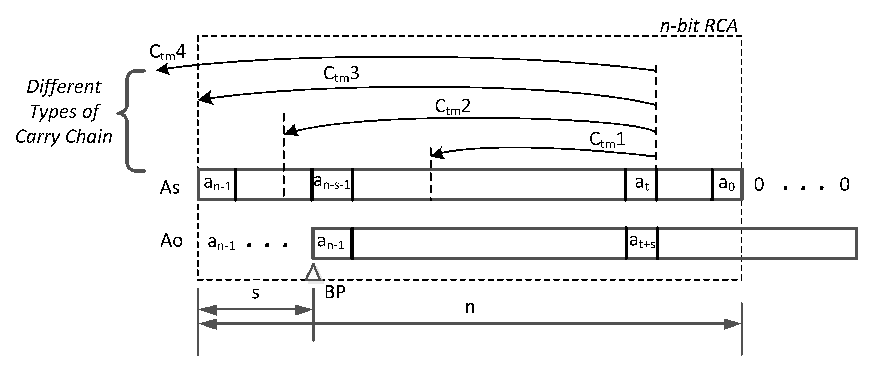
\includegraphics[width=3.3in]{./Figures/CCM_DataFlow3.eps}
%  \vspace{-2ex}
  \caption{Different types of carry chain in constant coefficient multiplier. The notion $s$ denotes the shifted bits and $BP$ denotes the binary point.}
  \label{CCM_fig}
%  \vspace{-1.5ex}
\end{figure}

\subsection{Probabilistic Model of Truncation Error}
Let $E_{Tin}$ and $E_{Tout}$ denote the expectation of truncation error at the input and output of CCM respectively. We then have (\ref{Et_CCM}), where $coe$ denotes the coefficient value of the CCM, and $E_{Tin}$ can be obtained according to~(\ref{TruncationError}).
%
\begin{eqnarray}\label{Et_CCM}
%\vspace{-1ex}
%\small
%\footnotesize
%\scriptsize
  E_{Tout}=|coe|\cdot E_{Tin}
%  \vspace{-1ex}
\end{eqnarray}
%\normalsize

\subsection{Probabilistic Model of Overclocking Error}
\subsubsection{Absolute Value of Overclocking Error}
The absolute value of overclocking error of carry chain $C_{tm}$ is increased by a factor of $2^s$ due to shifting, compared to RCA. Hence $e_{tm}$ in CCM can be modified from (\ref{etm}) to give (\ref{etm_CCM}).
%
\begin{eqnarray}\label{etm_CCM}
%\vspace{-1ex}
%\small
%\footnotesize
  e_{tm}=2^{t+b-n+s}
%  \vspace{-1.5ex}
\end{eqnarray}
%\normalsize

\subsubsection{Probability of Overclocking Error}
Due to the dependencies in a CCM, carry generation requires $a_t=a_{t-s}=1$, propagation and annihilation of a carry chain is best considered separately for four types of carry chain generated at bit~$t$. We label these by $C_{tm}1$ to $C_{tm}4$ in Figure~\ref{CCM_fig}, defined by the end region of the carry chain. For $C_{tm}1$, we have:
\begin{itemize}
  \item Carry propagation: $\!a_i\neq\!a_{i+s}\!$ where $\!i\!\in[t+1,n-s-2]\!$;
  \item Carry annihilation: $\!a_j\!=\!a_{j+s}\!$ where $\!j\!\in[t+1,n-s-1]\!$.
\end{itemize}
Similarly for $C_{tm}2$, we have:
\begin{itemize}
  \item Carry propagation: $a_i\neq a_{n-1}$ where $i\in[n-s-1,n-3]$; or $a_i\neq a_{i+s}$ where $i\in[t+1,n-s-2]$;
  \item Carry annihilation: $\!a_j\!=a_{n-1}\!$ where $j\!\in\![n-s-1,n-2]$.
\end{itemize}

For the first two types of carry chain $C_{tm}1$ and $C_{tm}2$, the probability of carry propagation and annihilation is $1/2$ and the probability of carry generation is $1/4$, under the premise that all bits of input signal are mutually independent. Therefore (\ref{Ptm_CCM1}) can be obtained by substituting this into~(\ref{Ptm_RCA}).
%
\begin{eqnarray}\label{Ptm_CCM1}
%\vspace{-1ex}
%\small
%\footnotesize
  P_{tm}=\left(1/2\right)^{m+1}, & \textrm{if $t+m-1\leqslant n-2$}
\end{eqnarray}
%\normalsize

For carry annihilation of $C_{tm}3$, $a_{n-1}=a_{n-1}$, which is always true. Thus the probability of $C_{tm}3$ is given by (\ref{Ptm_CCM2}).
%
\begin{eqnarray}\label{Ptm_CCM2}
%\vspace{-1ex}
%\small
%\footnotesize
  P_{tm}=\left(1/2\right)^m, & \textrm{if $t+m-1=n-1$}
%  \vspace{-1ex}
\end{eqnarray}
%\normalsize
$C_{tm}4$ represents carry chain annihilates over $a_{n-1}$, therefore carry propagation requires $a_{n-1}\neq a_{n-1}$. This means $C_{tm}4$ never occurs in a CCM.

Altogether, $P_{tm}$ for a CCM is given by (\ref{Ptm_CCM}).
\begin{eqnarray}\label{Ptm_CCM}
%\small
  P_{tm}=\left\{\begin{array}{ll}
      (1/2)^{m+1} & \textrm{if $t+m-1<n-1$}\\
      (1/2)^{m} & \textrm{if $t+m-1=n-1$}
    \end{array} \right.
    %\vspace{-1ex}
\end{eqnarray}
%\normalsize

\subsubsection{Expectation of Overclocking Error}
Since the carry chain of a CCM will not propagate over $a_{n-1}$, the upper bound of parameter $t$ and $m$ should be modified from (\ref{t_RCA}) and (\ref{m_RCA}) to give (\ref{t_CCM}) and (\ref{m_CCM}).
%
\begin{eqnarray}
%\vspace{-1ex}
%\small
%\footnotesize
%\scriptsize
  \label{t_CCM} 0\leqslant t\leqslant n-b-1\\
  \label{m_CCM} b<m\leqslant n-t
%  \vspace{-1ex}
\end{eqnarray}
%\normalsize

Finally, by substituting (\ref{Ptm_CCM}) and (\ref{etm_CCM}) with modified bounds of $t$ and $m$ into (\ref{Eo_exp}), we obtain the expectation of overclocking error for a CCM to be given by (\ref{Eo_CCM}).
%
\begin{eqnarray}\label{Eo_CCM}
%\vspace{-1ex}
%\small
%\footnotesize
      E_O=\left\{
        \begin{matrix}
            2^{s-b-1}-2^{s-n-1}, & \textrm{if $b\leq n-1$}\\
            0, & \textrm{otherwise}
        \end{matrix}
      \right.
%      \vspace{1ex}
\end{eqnarray}
%\normalsize

\subsection{CCM with Multiple RCAs and Shifters}\label{CCM_Multi}
In the case where a CCM is composed of two shifters and one RCA, such as operation $\!B\!=\!20A\!=\!(\!A<<2)+(\!A<<4)$, let the shifted bits be denoted as $s_1$ and $s_2$ respectively. Hence the equivalent $s$ in (\ref{Eo_CCM}) can be obtained through~(\ref{ShiftNo}).
%
%\vspace{-3ex}
\begin{eqnarray}\label{ShiftNo}
%\footnotesize
%\scriptsize
  s=\left|s_1-s_2\right|
%  \vspace{-1ex}
\end{eqnarray}

For those operations such as $B=37A=(A<<5)+(A<<2)+(A<<1)$, the CCM can be built using a tree structure. Each root node is the baseline CCM and the errors are propagated through an adder tree, of which the error can be determined based on our previous RCA model.

\section{Carry Select Adder}
\subsection{Introduction}
Since the delay of RCA is determined by the length of carry chain, there are several alternative adder architectures proposed to shorten the carry chain. For instance, the carry select adder (CSA) is designed to overlap carry propagation in sections such that the operating speed can be boosted. In a CSA, the carry chain is divided into multiple stages. Each stage contains two RCAs and two multiplexers. For a given input, computations are performed twice simultaneously, with the carry input as zero and one respectively. The results are then selected according to the actual carry input. Although this structure brings timing benefits, it costs extra hardware resources than RCA as the carry chain is duplicated and multiplexers are expensive especially in the FPGA technology. In this section, silicon area is incorporated as the third metric besides accuracy and performance. We explore the trade-offs between these three factors for both adder structures. The objective is to demonstrate the best design choice for a given set of design constraints.

%\begin{figure*}[t]
%  \centering
%  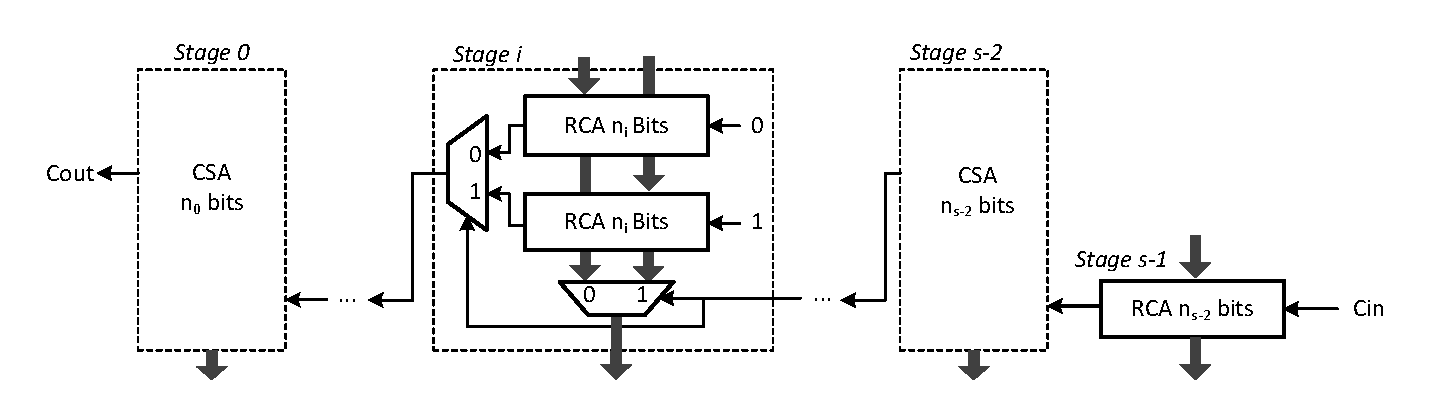
\includegraphics[width=\textwidth]{./Figures/CSAstructure.pdf}
%  \caption{Structure of an $s$-stage CSA.}
%\end{figure*}

%In addition to RCA, there are several

\subsection{Timing Models for Carry Select Adder}
We initially describe the modelling method for the CSA timing, with the aim of forming the relationship between the operating frequency and the corresponding maximum word-length of CSA. This information can be employed to determine the truncation error based on the models presented in Section.xxx.

In a CSA with $s$ stages~($s\geqslant 2$), let the stage delay be denoted by $d_{0}\dots d_{s-1}$, where $d_{0}$ and $d_{s-1}$ represent the delay of the most significant stage and the least significant stage, respectively. Unlike other stages, the least significant stage is built by one RCA only, since it is directly driven by the carry input. In our analysis, we follow the previous assumption that delay is due to carry propagation as well as, in this case, multiplexing the carry output. Therefore the delay of the $i^{th}$ stage can be obtained through~(\ref{CSA_SingleStageDelay}), where $\mu_{c}$ denotes the delay of $1$-bit carry propagation and $\mu_{mux}$ denotes the delay of multiplexing.
%Note that the delay of the ${(s-1)}^{th}$ and ${(s-2)}^{th}$ stages are identical, because the least significant stage of CSA is built by RCA.
\begin{eqnarray}\label{CSA_SingleStageDelay}
  d_i=\left\{
    \begin{matrix}
      n_i\cdot \mu_{c}+(i+1)\cdot\mu_{mux}, &\textrm{if $i\in\left[0,s-2\right]$}\\
      d_{i-1}, & \textrm{if $i=s-1$}
    \end{matrix}
  \right.
\end{eqnarray}

Under the timing-driven design environment, the delay of each stage of CSA is set to be approximately uniform for the fastest operation. In this case we obtain~(\ref{CSA_DelayEqual}).
\begin{eqnarray}\label{CSA_DelayEqual}
  d_0=d_1=\cdots=d_{s-1}
\end{eqnarray}

Substituting (\ref{CSA_SingleStageDelay}) into (\ref{CSA_DelayEqual}) yields (\ref{CSA_DelayRep}), which denotes the CSA word-length of stage $i$.
%Note that the word-length of stage $s-1$ and $s-2$ are identical, since the least significant stage is composed of RCA.
\begin{eqnarray}\label{CSA_DelayRep}
 n_i=\left\{
	\begin{matrix}
	  n_0-i\cdot\frac{\mu_{mux}}{\mu_c}, & \textrm{if $i\in\left[0,s-2\right]$}\\
	  n_{i-1}, &\textrm{if $i=s-1$}
      %n_0-(c-2)\cdot\frac{\mu_{mux}}{\mu_c}, & \textrm{if $i=c-1$ and $c\geqslant2$}
	\end{matrix}
    \right.
\end{eqnarray}

The word-length of CSA is then given by (\ref{CSA_WL}).
\begin{eqnarray}\label{CSA_WL}
  n_{CSA}=\sum_{i=0}^{s-1}n_{i}=s\cdot n_{0}-\frac{\mu_{mux}}{\mu_{c}}\cdot\frac{(s+1)(s-2)}{2}
\end{eqnarray}

In the conventional situation, the word-length of both RCA and CSA should be properly selected in order to meet timing. In this case,~(\ref{CSA_RCA}) can be obtained, where $n_{RCA}$ is determined by current timing information through (xxx).
\begin{eqnarray}\label{CSA_RCA}
  \mu_{c}\cdot n_{RCA}=\mu_{c}n_0+\mu_{mux}
\end{eqnarray}

Based on~(\ref{CSA_WL}) and~(\ref{CSA_RCA}), we may obtain the representation of the word-length of CSA in terms of a given timing constraint, as presented in~(\ref{CSA_Timing}).
% we form the relationship between the word-length of CSA and RCA under a given timing constraint, as presented in~(\ref{CSA_Timing}).
\begin{eqnarray}\label{CSA_Timing}
  n_{CSA}=s\cdot n_{RCA}-\frac{\mu_{mux}}{\mu_{c}}\cdot\frac{(s+2)(s-1)}{2}
\end{eqnarray}

It can be seen that $s=1$ leads to $n_{CSA}=n_{RCA}$. This is because RCA forms the least significant stage of CSA. In addition, combine (\ref{CSA_DelayRep}) and (\ref{CSA_RCA}) to ensure $n_{s-1}>0$, we obtain the upper bond of the stage number by~(\ref{CSA_StageNumber}).
\begin{eqnarray}\label{CSA_StageNumber}
  s<n_{RCA}\cdot\frac{\mu_c}{\mu_{mux}}+1
\end{eqnarray}
%the word-length of each CSA stage is allocated to ensure that

\subsection{Model Verification}
As seen in (\ref{CSA_Timing}), the value of $\mu_{mux}/\mu_c$ should be determined before applying the timing model. This ratio can be obtained through timing analysis. Specifically, varying the word-length of a single stage $n_i$ and recording the corresponding delay value $d_i$ through the timing analysis tool. According to~(\ref{CSA_SingleStageDelay}), the ratio can be obtained by fitting those values using linear polynomials.
%, as presented in Fig.~(\ref{DelayFitting}). Out experimental results show that $\mu_{mux}/\mu_c\approx8$.
%
%\begin{figure}[htbp]
%  \centering
%  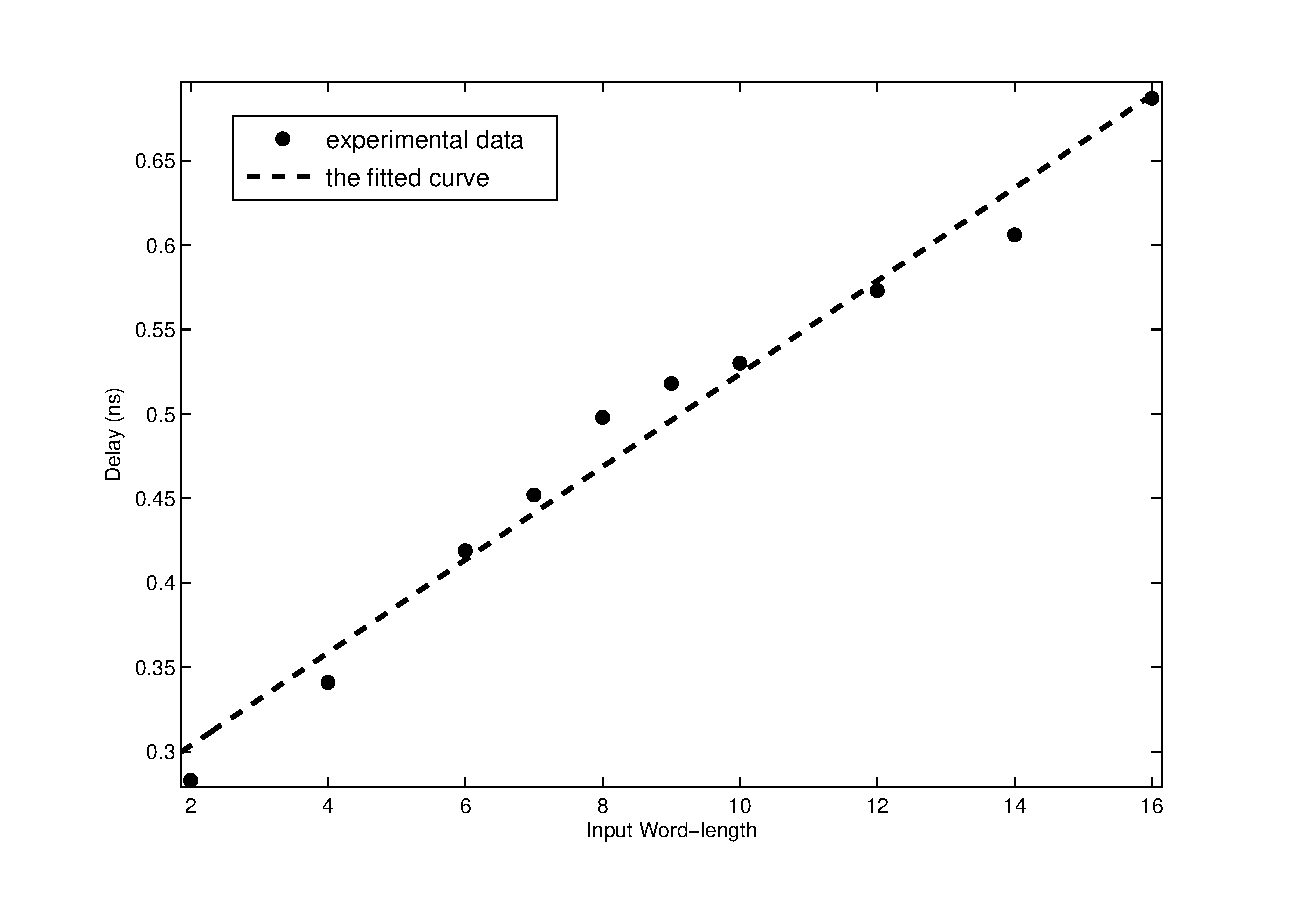
\includegraphics[width=3.3in]{./Figures/Fitting.eps}
%  \caption{Fitted curve of (\ref{CSA_SingleStageDelay}) for the most significant stage ($i=0$), based on the given input word-length and the corresponding delay value obtained through the Xilinx Timing Analyzer.}
%  \label{DelayFitting}
%\end{figure}

Using this information, we verify our timing model with experimental results, which are obtained from post place and route simulations on Xilinx Virtex-6 FPGAs. Fig.~\ref{CSA Model Verification} demonstrates both the modelled value and the experimental results of the maximum word-length of the 2-stage CSA for various operating frequencies. In this experiment, the input data are randomly sampled from a 16-bit data set, which follows uniform distribution. It can be seen that the the modelled value match well with the experimental results.
%The maximum input word-length in our experiments is 16-bit, hence the modelled value is set to 16 if it expires.
\begin{figure}[htbp]
  \centering
  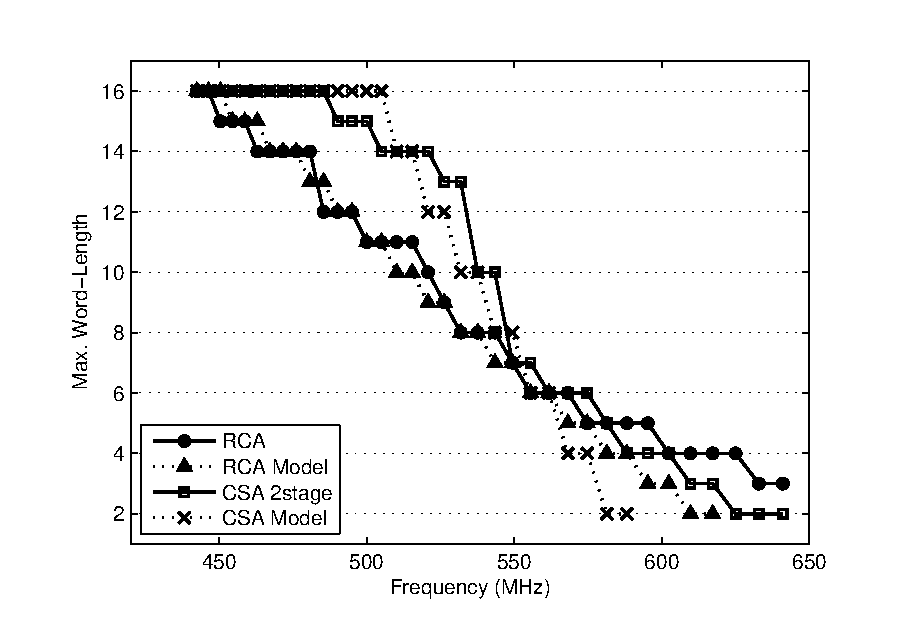
\includegraphics[width=3in]{./Figures/Model.eps}
  \caption{Comparison of the maximum word-length for a given operating frequency between the modelled value and the experimental results from FPGA simulations.}
  \label{CSA Model Verification}
\end{figure}

%It can be seen that our timing models match well the experimental results for both RCA and CSA, except that the modelled outcomes are slight conservative, especially at higher operating frequencies. This is because the model coefficients are obtained based on timing analysis, which is designed with safety margins to ensure correct functionality for diverse operating conditions. In addition, routing delay might be introduced during timing analysis such that the overall delay is enlarged, while our models consider logic delay only.

\subsection{Area Overhead}
Fig.~\ref{CSA3stage Timing} demonstrates the maximum word-lengths for RCA and CSA with 2 stages and 3 stages under a range of operating frequencies. We only investigate 3 stages as the maximum stages number predicted in (\ref{CSA_StageNumber}) is 3. It can be seen that in comparison to RCA, CSA achieves greater word-length when frequency is initially increased. This corresponds to smaller truncation errors. RCA only outperforms than CSA when very high frequency is applied. In addition, the word-length of 3-stage CSA is always greater than 2-stage CSA across the entire frequency domain, as expected.
%\begin{figure}[htbp]
%  \centering
%  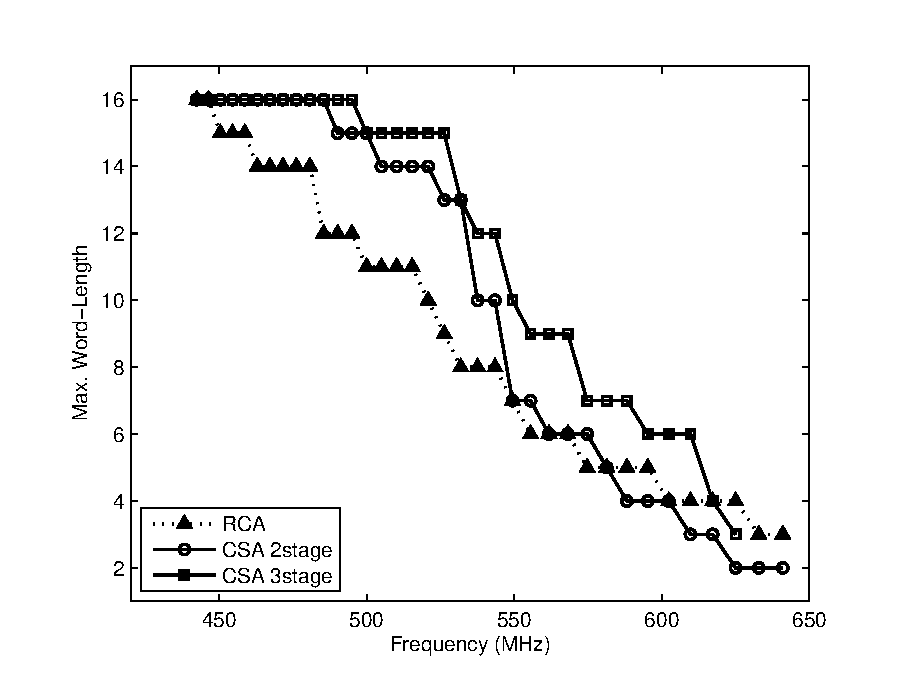
\includegraphics[width=3.3in]{./Figures/CSA3stage_Timing.eps}
%  \caption{Maximum word-length for RCA and CSA across a variety of frequencies.}
%  \label{CSA3stage Timing}
%\end{figure}

\begin{figure}[htbp]
    \begin{minipage}[b]{.48\textwidth}
        \centering
        \subfigure[Maximum word-length.]{
            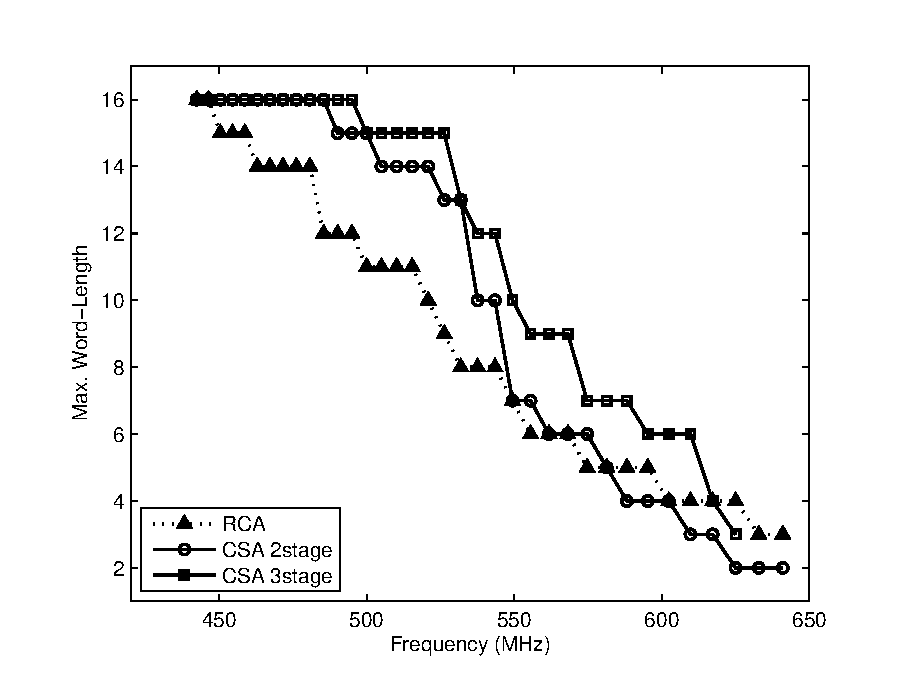
\includegraphics[width=3.3in]{./Figures/CSA3stage_Timing.eps}
            \label{CSA3stage Timing}
        }
        \subfigure[Hardware resource usage.]{
            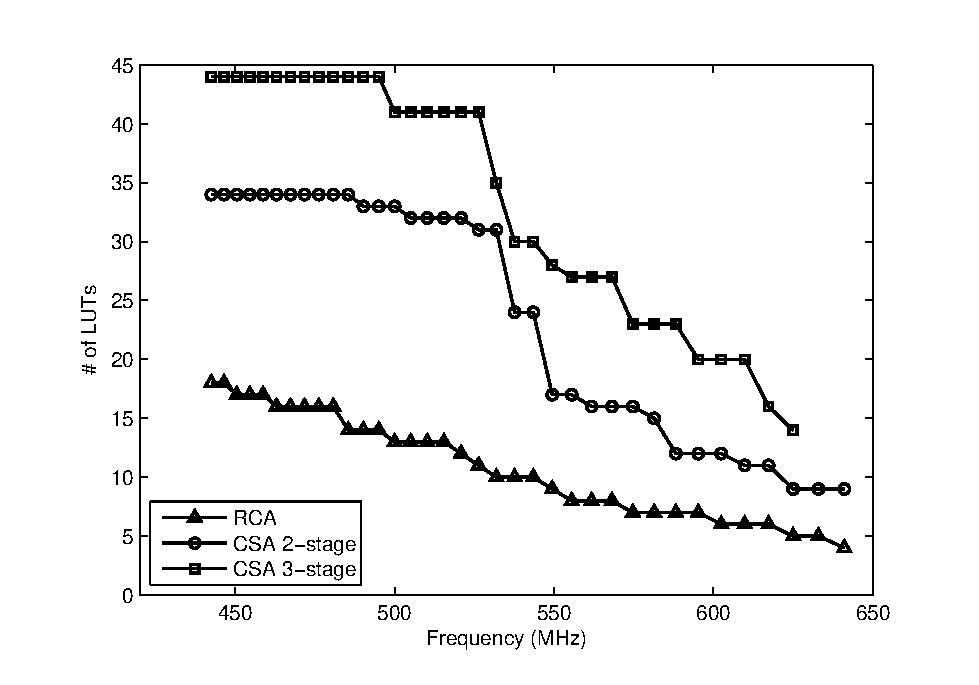
\includegraphics[width=3.3in]{./Figures/CSA3stage_Area.eps}
            \label{CSA3stage Area}
        }
    \end{minipage}
    \centering
    \caption{Comparison between RCA and CSA across a variety of frequency values in terms of the maximum word-length of input signal and the area consumption.}
\end{figure}

However, the accuracy benefits brought by CSA comes with the cost of large area overhead. Fig.~\ref{CSA3stage Area} depicts the resource usage (in terms of the number of Look-Up Tables (LUTs) in the FPGA) used for all three structures. It can be seen that for a given frequency, the 3-stage CSA consumes $2.4\times\sim3.7\times$ area than RCA, while the number of the 2-stage CSA is $1.7\times\sim3.1\times$. This finding poses a question of whether CSA with higher stage numbers still offer better accuracy than RCA under a limited area budget.
%\begin{figure}[htbp]
%  \centering
%  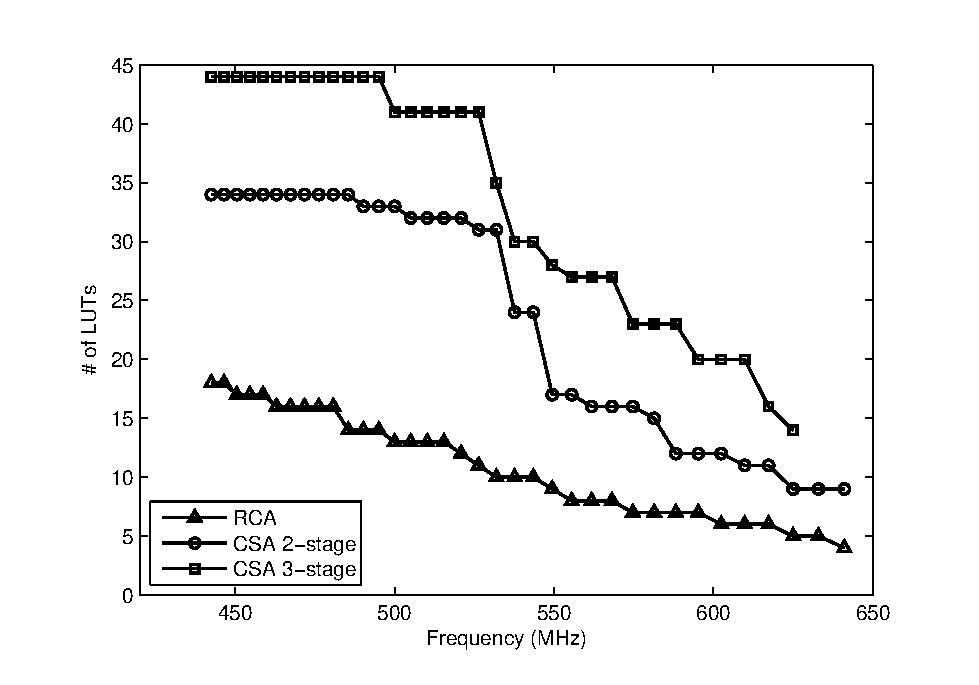
\includegraphics[width=3.3in]{./Figures/CSA3stage_Area.eps}
%  \caption{Area overhead for RCA and CSA.}
%  \label{CSA3stage Area}
%\end{figure}

\subsection{Exploring Trade-offs Between Accuracy, Performance and Area}
%Although advanced architectures such as CSA inherently offer better performance than the basic structure, this would generate a large area overhead. In the following experiments,
To answer this question, we explore the trade-offs between accuracy, performance as well as area in this section. If the available hardware resources are limited, the full word-length of both CSA and RCA might not be implemented. The precision lose might generates large errors even at low frequencies. This is demonstrated by experiments where area constraints are applied besides the timing requirement. Conventionally, both of the constraints are met by reducing the word-length of the input signal. The errors at the outputs are recorded with the reference to the original word-length, which is 16 bits in the following experiments. In addition, we propose another designing method where RCA is implemented with the maximum possible word-length under the given area budget, while the timing constraints are met by overclocking. For a certain pair of $\{Area, Frequency\}$ constraint, the optimum design method is selected based on the following criteria:
%For instance, Fig.xxx to Fig.xxx illustrate error expectations of all the described design scenarios when setting the LUTs number to 45, 35, 25 and 15 respectively. The optimal design metric with the minimum error expectation is labelled for each area constraint. For a given frequency and area constraint, the optimum design is chosen based on the following metrics:
\begin{itemize}
  \item Design with the minimum error expectation is the optimum design;
  \item If multiple designs achieve the same error expectation, then the design with minimum area is the optimum design;
  \item If the error expectation and area are identical for multiple designs, they are all treated as the optimum design.
\end{itemize}

The optimum design method for a variety of frequency and area constraints is demonstrated in Fig.~\ref{Tradeoff}, from which several observations can be made. If the available area is large enough, CSA serves as the optimum design option because it inherently operates faster than RCA, and it can be implemented with full precision in this situation. The 2-stage CSA is better than the 3-stage CSA when frequency is initially increased, as it consumes less area although both of them achieve the same error expectation. For a tighter area budget, only part of the CSA can be implemented, whilst RCA still keeps full precision. In this case, area instead of timing becomes the dominate factor for small frequency values. This leads to precision loss for CSA initially. Therefore we see RCA with overclocking is the best design across almost the whole frequency domain. For an even stringent area constraint, the word-length of RCA is also limited. This results in truncation error initially for all design scenarios. Meanwhile, CSA with high stage numbers could not even be implemented at all. 
\begin{figure}[htbp]
  \centering
  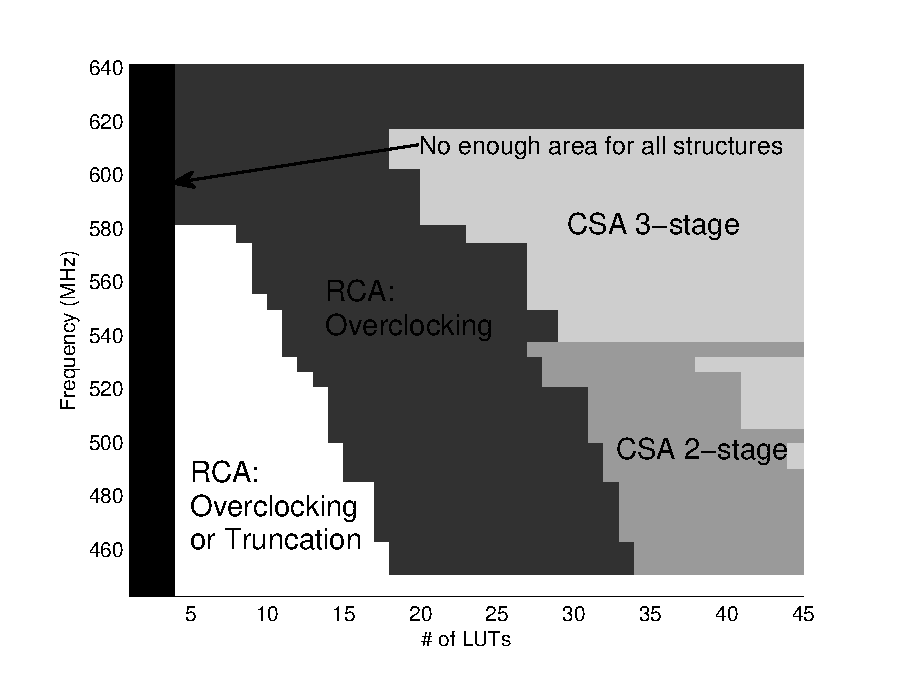
\includegraphics[width=3.5in]{./Figures/Tradeoff.eps}
  \caption{Demonstration of the optimum design methodology for a variety frequency and area constraints.}
  \label{Tradeoff}
\end{figure}

%We also notice that for small frequencies, RCA with either overclocking or truncation of word-length of the input signal is the best design choice for any area constraint, since 

%\begin{figure}[htbp]
%	\centering
%	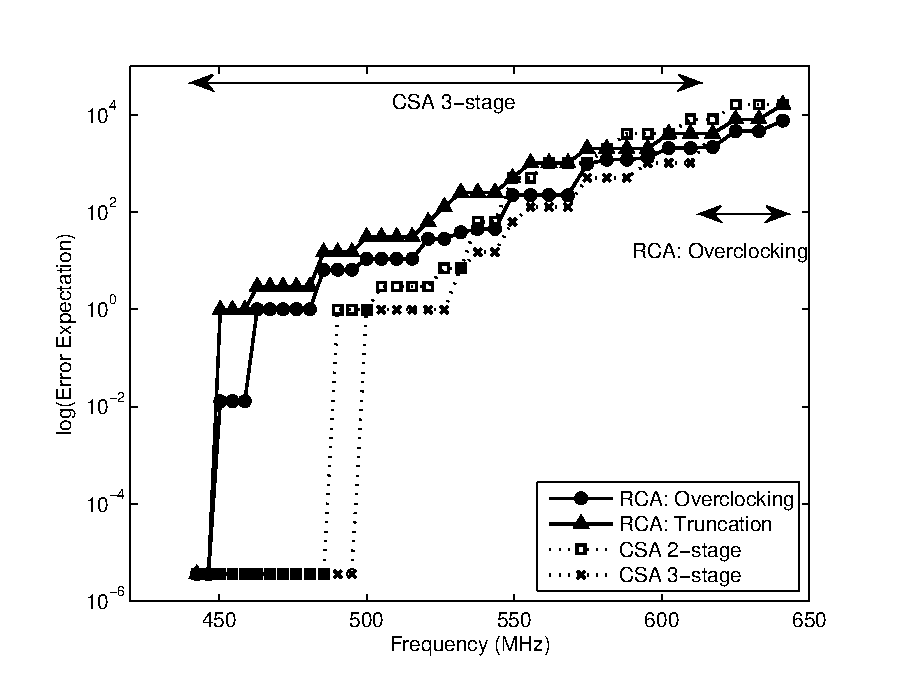
\includegraphics[width=3.3in]{./Figures/Error_LUT45.eps}
%	\caption{LUT=45}
%\end{figure}
%
%\begin{figure}[htbp]
%	\centering
%	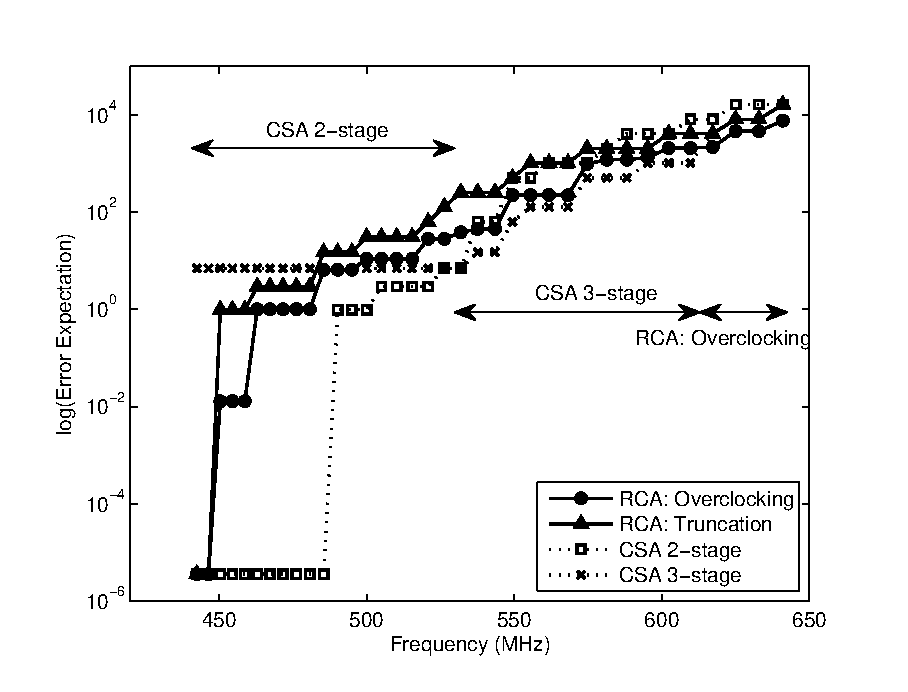
\includegraphics[width=3.3in]{./Figures/Error_LUT35.eps}
%	\caption{LUT=35}
%\end{figure}
%
%\begin{figure}[htbp]
%	\centering
%	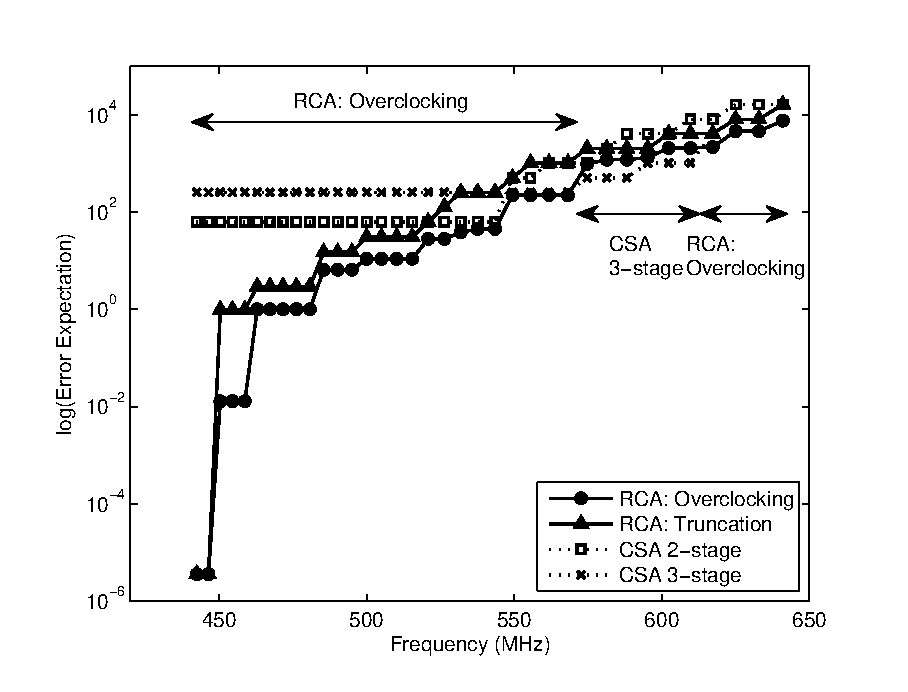
\includegraphics[width=3.3in]{./Figures/Error_LUT25.eps}
%	\caption{LUT=25}
%\end{figure}
%
%\begin{figure}[htbp]
%	\centering
%	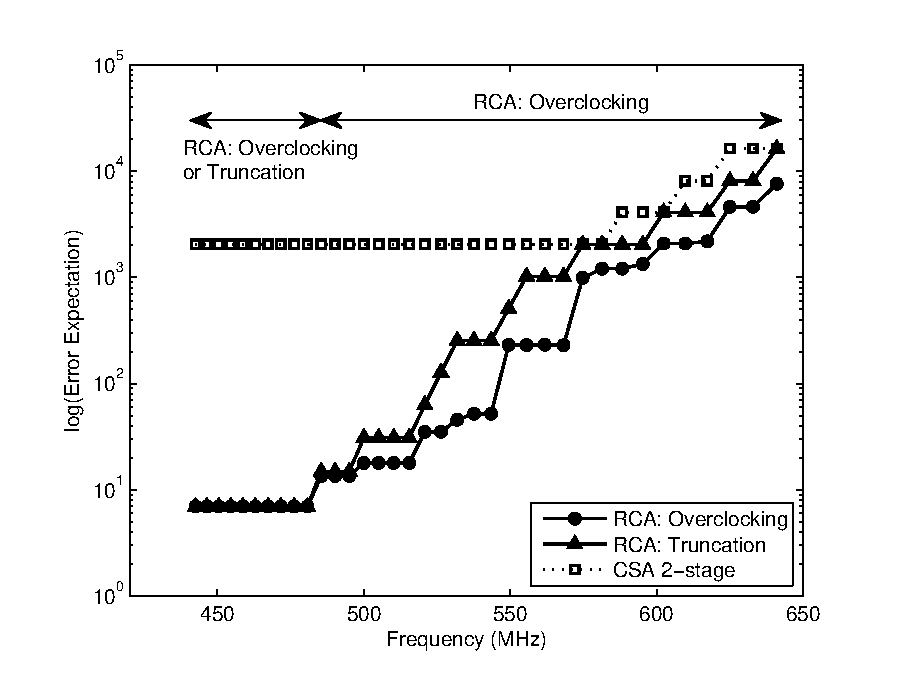
\includegraphics[width=3.3in]{./Figures/Error_LUT15.eps}
%	\caption{LUT=15}
%\end{figure}
%
%If the available area is large enough, as shown in Fig.xxx, CSA with higher stage numbers can be implemented with full precision and it is the optimal design choice unless very high frequencies are applied. This is because at lower frequencies, the long carry chain is divided into multiple overlapped sections, and the higher stage number the shorter the carry chain length of each stage. When the frequency increases, however, the multiplexer delay becomes comparable to the carry chain delay, and this will limit the maximum word-length of CSA. It can be seen that the overclocked RCA achieves best accuracy at higher frequencies.

%For a tighter area budget, only part of the complex structures can be implemented, whilst the simple structure still keeps full precision. As can be seen in Fig.xxx and Fig.xxx, area instead of timing becomes the dominate factor when frequency is initially increased. This lead to a large truncation error for both 2-stage and 3-stage CSA. In this situation, overclocking RCA serves as the optimum choice with respect to accuracy.

%In general, the error expectations at the output of all four design method for a set of timing and area constraints are demonstrated in Fig.~\ref{Tradeoff}, from which several observations can be made.



% An example of a floating figure using the graphicx package.
% Note that \label must occur AFTER (or within) \caption.
% For figures, \caption should occur after the \includegraphics.
% Note that IEEEtran v1.7 and later has special internal code that
% is designed to preserve the operation of \label within \caption
% even when the captionsoff option is in effect. However, because
% of issues like this, it may be the safest practice to put all your
% \label just after \caption rather than within \caption{}.
%
% Reminder: the "draftcls" or "draftclsnofoot", not "draft", class
% option should be used if it is desired that the figures are to be
% displayed while in draft mode.
%
%\begin{figure}[!t]
%\centering
%\includegraphics[width=2.5in]{myfigure}
% where an .eps filename suffix will be assumed under latex,
% and a .pdf suffix will be assumed for pdflatex; or what has been declared
% via \DeclareGraphicsExtensions.
%\caption{Simulation Results.}
%\label{fig_sim}
%\end{figure}

% Note that IEEE typically puts floats only at the top, even when this
% results in a large percentage of a column being occupied by floats.


% An example of a double column floating figure using two subfigures.
% (The subfig.sty package must be loaded for this to work.)
% The subfigure \label commands are set within each subfloat command,
% and the \label for the overall figure must come after \caption.
% \hfil is used as a separator to get equal spacing.
% Watch out that the combined width of all the subfigures on a
% line do not exceed the text width or a line break will occur.
%
%\begin{figure*}[!t]
%\centering
%\subfloat[Case I]{\includegraphics[width=2.5in]{box}%
%\label{fig_first_case}}
%\hfil
%\subfloat[Case II]{\includegraphics[width=2.5in]{box}%
%\label{fig_second_case}}
%\caption{Simulation results.}
%\label{fig_sim}
%\end{figure*}
%
% Note that often IEEE papers with subfigures do not employ subfigure
% captions (using the optional argument to \subfloat[]), but instead will
% reference/describe all of them (a), (b), etc., within the main caption.


% An example of a floating table. Note that, for IEEE style tables, the
% \caption command should come BEFORE the table. Table text will default to
% \footnotesize as IEEE normally uses this smaller font for tables.
% The \label must come after \caption as always.
%
%\begin{table}[!t]
%% increase table row spacing, adjust to taste
%\renewcommand{\arraystretch}{1.3}
% if using array.sty, it might be a good idea to tweak the value of
% \extrarowheight as needed to properly center the text within the cells
%\caption{An Example of a Table}
%\label{table_example}
%\centering
%% Some packages, such as MDW tools, offer better commands for making tables
%% than the plain LaTeX2e tabular which is used here.
%\begin{tabular}{|c||c|}
%\hline
%One & Two\\
%\hline
%Three & Four\\
%\hline
%\end{tabular}
%\end{table}


% Note that IEEE does not put floats in the very first column - or typically
% anywhere on the first page for that matter. Also, in-text middle ("here")
% positioning is not used. Most IEEE journals use top floats exclusively.
% Note that, LaTeX2e, unlike IEEE journals, places footnotes above bottom
% floats. This can be corrected via the \fnbelowfloat command of the
% stfloats package.



\section{Conclusion}
The conclusion goes here.







% use section* for acknowledgement
\section*{Acknowledgment}


The authors would like to thank...


% Can use something like this to put references on a page
% by themselves when using endfloat and the captionsoff option.
\ifCLASSOPTIONcaptionsoff
  \newpage
\fi



% trigger a \newpage just before the given reference
% number - used to balance the columns on the last page
% adjust value as needed - may need to be readjusted if
% the document is modified later
%\IEEEtriggeratref{8}
% The "triggered" command can be changed if desired:
%\IEEEtriggercmd{\enlargethispage{-5in}}

% references section

% can use a bibliography generated by BibTeX as a .bbl file
% BibTeX documentation can be easily obtained at:
% http://www.ctan.org/tex-archive/biblio/bibtex/contrib/doc/
% The IEEEtran BibTeX style support page is at:
% http://www.michaelshell.org/tex/ieeetran/bibtex/
%\bibliographystyle{IEEEtran}
% argument is your BibTeX string definitions and bibliography database(s)
%\bibliography{IEEEabrv,../bib/paper}
%
% <OR> manually copy in the resultant .bbl file
% set second argument of \begin to the number of references
% (used to reserve space for the reference number labels box)
\begin{thebibliography}{1}

\bibitem{IEEEhowto:kopka}
H.~Kopka and P.~W. Daly, \emph{A Guide to \LaTeX}, 3rd~ed.\hskip 1em plus
  0.5em minus 0.4em\relax Harlow, England: Addison-Wesley, 1999.

\end{thebibliography}

% biography section
%
% If you have an EPS/PDF photo (graphicx package needed) extra braces are
% needed around the contents of the optional argument to biography to prevent
% the LaTeX parser from getting confused when it sees the complicated
% \includegraphics command within an optional argument. (You could create
% your own custom macro containing the \includegraphics command to make things
% simpler here.)
%\begin{IEEEbiography}[{\includegraphics[width=1in,height=1.25in,clip,keepaspectratio]{mshell}}]{Michael Shell}
% or if you just want to reserve a space for a photo:

\begin{IEEEbiography}{Author}
Biography text here.
\end{IEEEbiography}

% if you will not have a photo at all:
\begin{IEEEbiographynophoto}{Author}
Biography text here.
\end{IEEEbiographynophoto}

% insert where needed to balance the two columns on the last page with
% biographies
%\newpage

\begin{IEEEbiographynophoto}{Author}
Biography text here.
\end{IEEEbiographynophoto}

% You can push biographies down or up by placing
% a \vfill before or after them. The appropriate
% use of \vfill depends on what kind of text is
% on the last page and whether or not the columns
% are being equalized.

%\vfill

% Can be used to pull up biographies so that the bottom of the last one
% is flush with the other column.
%\enlargethispage{-5in}

\end{document}


